\chapter{Экспериментальные данные}\label{app:A}

\begin{figure}[!htbp]
    \centering
    \begin{adjustbox}{max totalsize={0.8\textwidth}{\textheight}}
        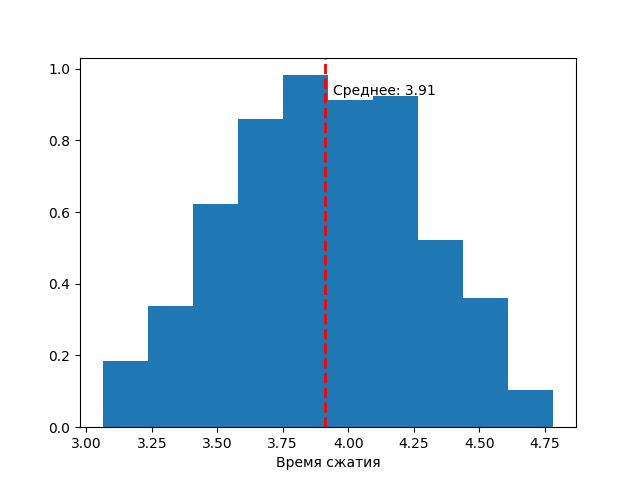
\includegraphics{images/hist-handmade-c-dev.png}
    \end{adjustbox}
    \caption{Время сжатия разработанным с нуля C-устройством.}\label{fig:hist-handmade-c-dev}
\end{figure}

{\tiny
\setlength\LTleft{-1.2cm}
    \begin{longtable}{|c|c|c|c|c|c|c|c|c|c|c|c|c|c|c|c|c|c|c|c|}%
        \caption{Время сжатия разработанным с нуля C-устройством.}\label{tbl:hist-handmade-c-dev} \\
        \hline
        № & $T$ &
        № & $T$ &
        № & $T$ &
        № & $T$ &
        № & $T$ &
        № & $T$ &
        № & $T$ &
        № & $T$ &
        № & $T$ &
        № & $T$ \\
        \hline
        \csvreader[column count=22,
                   no head,
                   table head=\hline,
                   late after line =\\\hline]{handmade-c-dev.csv}{
        1=\one, 2=\two, 3=\three, 4=\four,
        5=\five, 6=\six, 7=\seven, 8=\eight,
        9=\nine, 10=\ten, 11=\eleven, 12=\twelve,
        13=\thirteen, 14=\fourteen, 15=\fifteen, 16=\sixteen,
        17=\seventeen, 18=\eighteen, 19=\nineteen, 20=\twenty
        }
        {
            \one & \two &
            \three & \four &
            \five & \six &
            \seven & \eight &
            \nine & \ten &
            \eleven & \twelve &
            \thirteen & \fourteen &
            \fifteen & \sixteen &
            \seventeen & \eighteen &
            \nineteen & \twenty
        }
    \end{longtable}
}

\begin{figure}[!htbp]
    \centering
    \begin{adjustbox}{max totalsize={0.8\textwidth}{\textheight}}
        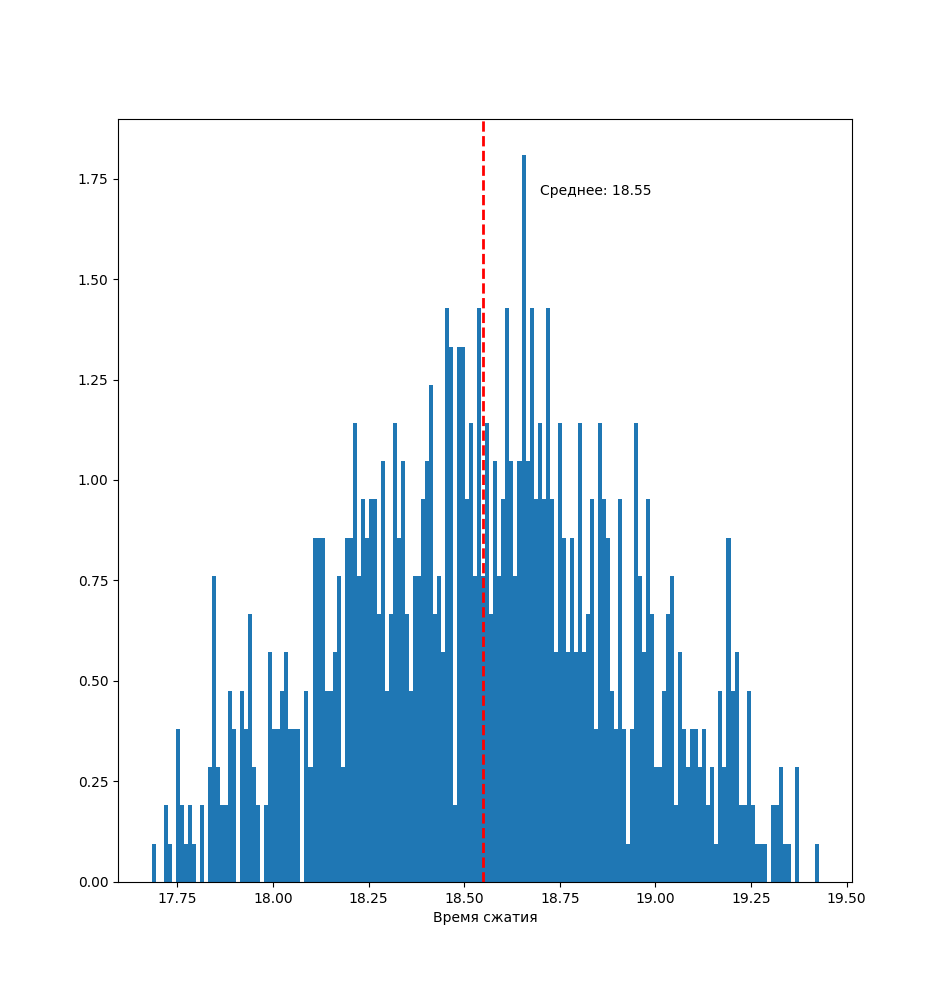
\includegraphics{images/hist-handmade-py-dev.png}
    \end{adjustbox}
    \caption{Время сжатия разработанным с нуля Python-устройством.}\label{fig:hist-handmade-py-dev}
\end{figure}

{\tiny
\setlength\LTleft{-1.5cm}
    \begin{longtable}{|c|c|c|c|c|c|c|c|c|c|c|c|c|c|c|c|c|c|c|c|}%
        \caption{Время сжатия разработанным с нуля Python-устройством.}\label{tbl:hist-handmade-py-dev} \\
        \hline
        № & $T$ &
        № & $T$ &
        № & $T$ &
        № & $T$ &
        № & $T$ &
        № & $T$ &
        № & $T$ &
        № & $T$ &
        № & $T$ &
        № & $T$ \\
        \hline
        \csvreader[column count=22,
                   no head,
                   table head=\hline,
                   late after line =\\\hline]{handmade-py-dev.csv}{
        1=\one, 2=\two, 3=\three, 4=\four,
        5=\five, 6=\six, 7=\seven, 8=\eight,
        9=\nine, 10=\ten, 11=\eleven, 12=\twelve,
        13=\thirteen, 14=\fourteen, 15=\fifteen, 16=\sixteen,
        17=\seventeen, 18=\eighteen, 19=\nineteen, 20=\twenty
        }
        {
            \one & \two &
            \three & \four &
            \five & \six &
            \seven & \eight &
            \nine & \ten &
            \eleven & \twelve &
            \thirteen & \fourteen &
            \fifteen & \sixteen &
            \seventeen & \eighteen &
            \nineteen & \twenty
        }
    \end{longtable}
}


\begin{figure}[!htbp]
    \centering
    \begin{adjustbox}{max totalsize={0.8\textwidth}{\textheight}}
        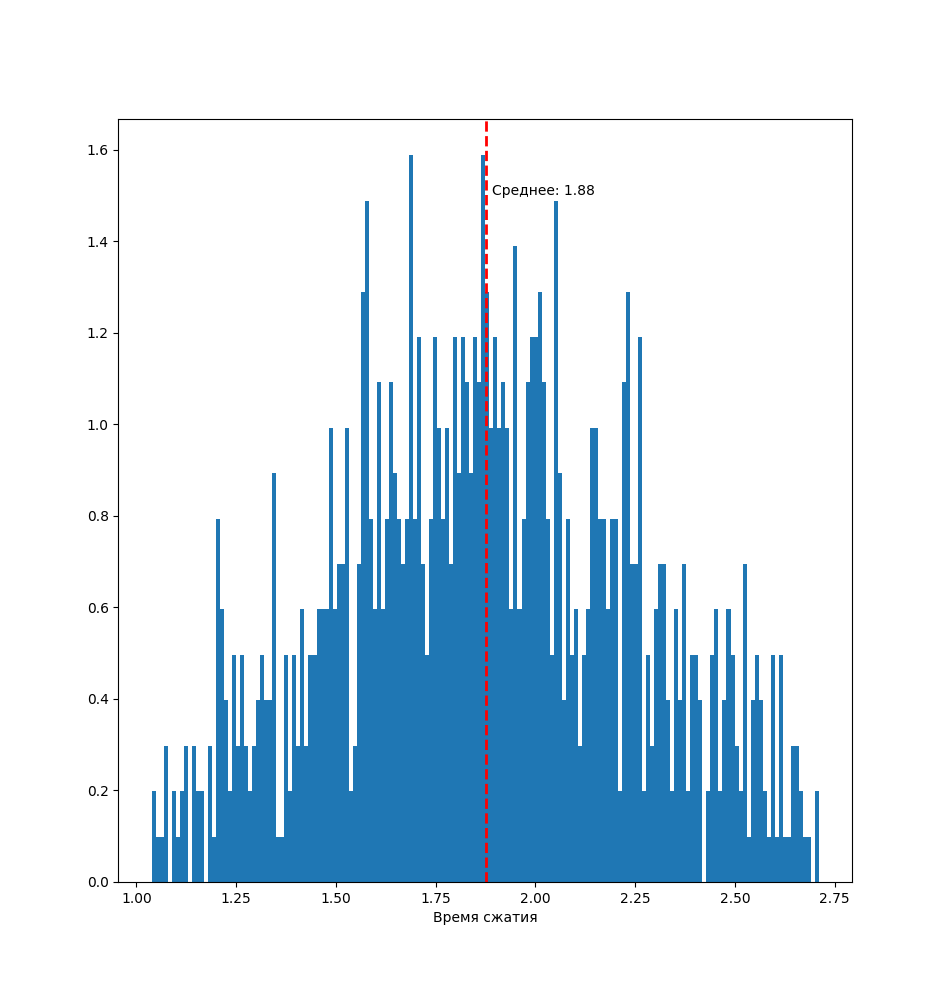
\includegraphics{images/hist-lib-c-dev.png}
    \end{adjustbox}
    \caption{Время сжатия C-устройством, использующим библиотеку сжатия.}\label{fig:hist-lib-c-dev}
\end{figure}

{\tiny
\setlength\LTleft{-1.2cm}
    \begin{longtable}{|c|c|c|c|c|c|c|c|c|c|c|c|c|c|c|c|c|c|c|c|}%
        \caption{Время сжатия C-устройством, использующим библиотеку сжатия.}\label{tbl:hist-lib-c-dev} \\
        \hline
        № & $T$ &
        № & $T$ &
        № & $T$ &
        № & $T$ &
        № & $T$ &
        № & $T$ &
        № & $T$ &
        № & $T$ &
        № & $T$ &
        № & $T$ \\
        \hline
        \csvreader[column count=22,
                   no head,
                   table head=\hline,
                   late after line =\\\hline]{lib-c-dev.csv}{
        1=\one, 2=\two, 3=\three, 4=\four,
        5=\five, 6=\six, 7=\seven, 8=\eight,
        9=\nine, 10=\ten, 11=\eleven, 12=\twelve,
        13=\thirteen, 14=\fourteen, 15=\fifteen, 16=\sixteen,
        17=\seventeen, 18=\eighteen, 19=\nineteen, 20=\twenty
        }
        {
            \one & \two &
            \three & \four &
            \five & \six &
            \seven & \eight &
            \nine & \ten &
            \eleven & \twelve &
            \thirteen & \fourteen &
            \fifteen & \sixteen &
            \seventeen & \eighteen &
            \nineteen & \twenty
        }
    \end{longtable}
}

\begin{figure}[!htbp]
    \centering
    \begin{adjustbox}{max totalsize={0.8\textwidth}{\textheight}}
        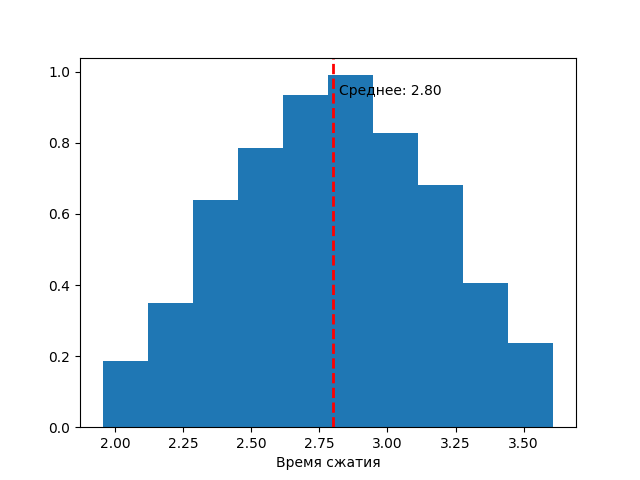
\includegraphics{images/hist-lib-py-dev.png}
    \end{adjustbox}
    \caption{Время сжатия Python-устройством, использующим библиотеку сжатия.}\label{fig:hist-lib-py-dev}
\end{figure}

{\tiny
\setlength\LTleft{-1.5cm}
    \begin{longtable}{|c|c|c|c|c|c|c|c|c|c|c|c|c|c|c|c|c|c|c|c|}%
        \caption{Время сжатия Python-устройством, использующим библиотеку сжатия.}\label{tbl:hist-lib-py-dev} \\
        \hline
        № & $T$ &
        № & $T$ &
        № & $T$ &
        № & $T$ &
        № & $T$ &
        № & $T$ &
        № & $T$ &
        № & $T$ &
        № & $T$ &
        № & $T$ \\
        \hline
        \csvreader[column count=22,
                   no head,
                   table head=\hline,
                   late after line =\\\hline]{lib-py-dev.csv}{
        1=\one, 2=\two, 3=\three, 4=\four,
        5=\five, 6=\six, 7=\seven, 8=\eight,
        9=\nine, 10=\ten, 11=\eleven, 12=\twelve,
        13=\thirteen, 14=\fourteen, 15=\fifteen, 16=\sixteen,
        17=\seventeen, 18=\eighteen, 19=\nineteen, 20=\twenty
        }
        {
            \one & \two &
            \three & \four &
            \five & \six &
            \seven & \eight &
            \nine & \ten &
            \eleven & \twelve &
            \thirteen & \fourteen &
            \fifteen & \sixteen &
            \seventeen & \eighteen &
            \nineteen & \twenty
        }
    \end{longtable}
}


\begin{figure}[!htbp]
    \centering
    \begin{adjustbox}{max totalsize={0.8\textwidth}{\textheight}}
        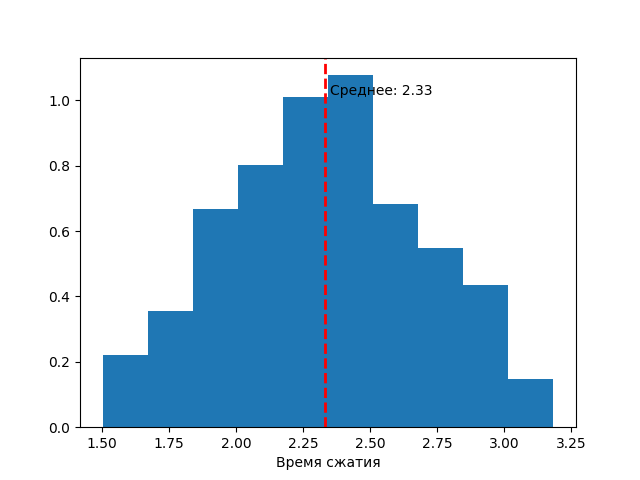
\includegraphics{images/hist-lib-c-network.png}
    \end{adjustbox}
    \caption{Время сжатия C-устройством по сети.}\label{fig:hist-lib-c-network}
\end{figure}


\begin{figure}[!htbp]
    \centering
    \begin{adjustbox}{max totalsize={0.8\textwidth}{\textheight}}
        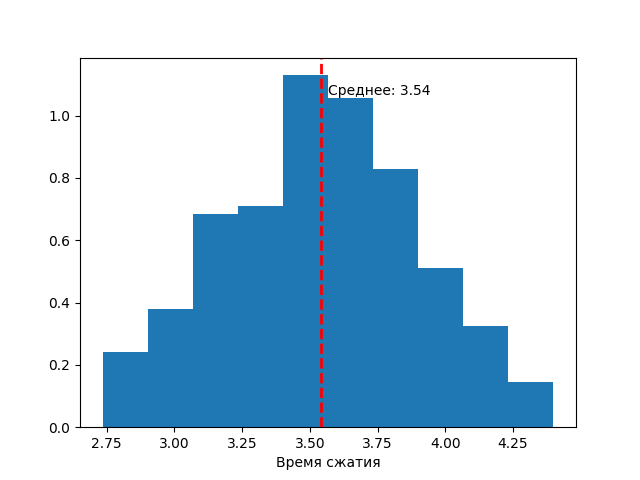
\includegraphics{images/hist-lib-py-network.png}
    \end{adjustbox}
    \caption{Время сжатия Python-устройством по сети.}\label{fig:hist-lib-py-network}
\end{figure}

\begin{figure}[!htbp]
    \centering
    \begin{adjustbox}{max totalsize={0.8\textwidth}{\textheight}}
        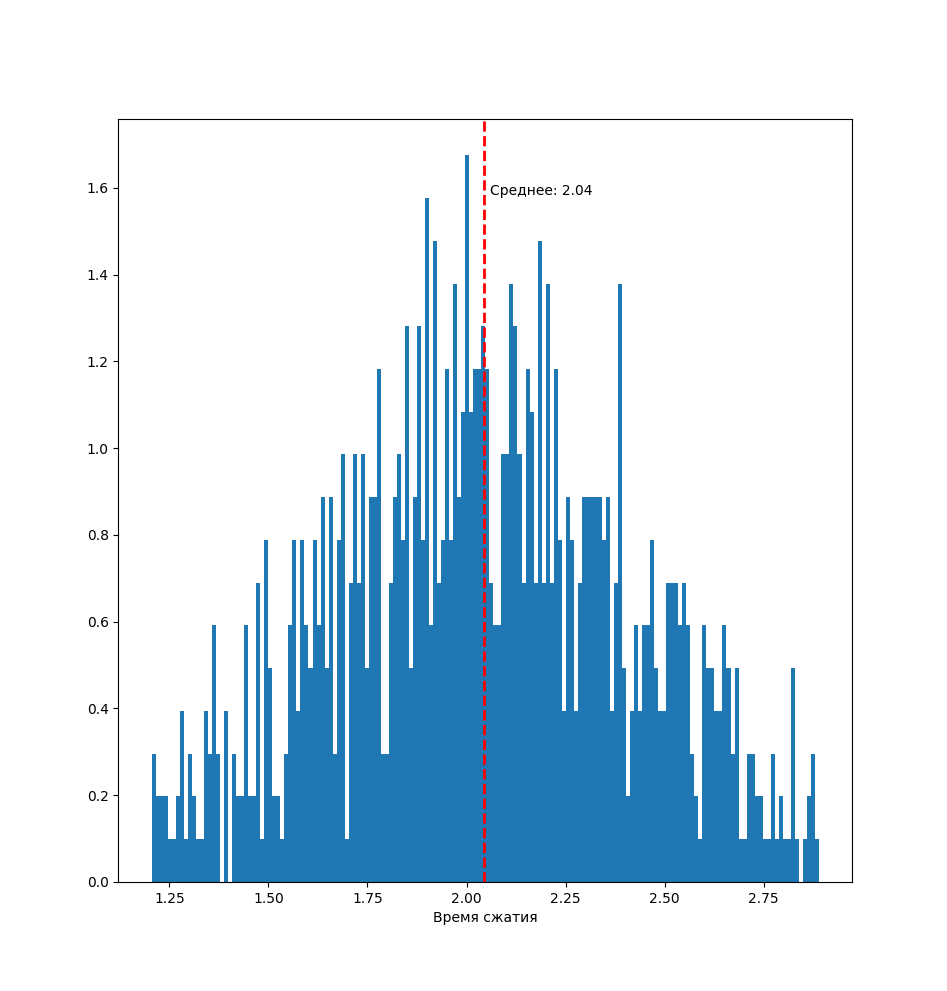
\includegraphics{images/hist-exec-c-dev.png}
    \end{adjustbox}
    \caption{Время сжатия C-устройством через подпроцесс.}\label{fig:hist-exec-c-dev}
\end{figure}

\begin{figure}[!htbp]
    \centering
    \begin{adjustbox}{max totalsize={0.8\textwidth}{\textheight}}
        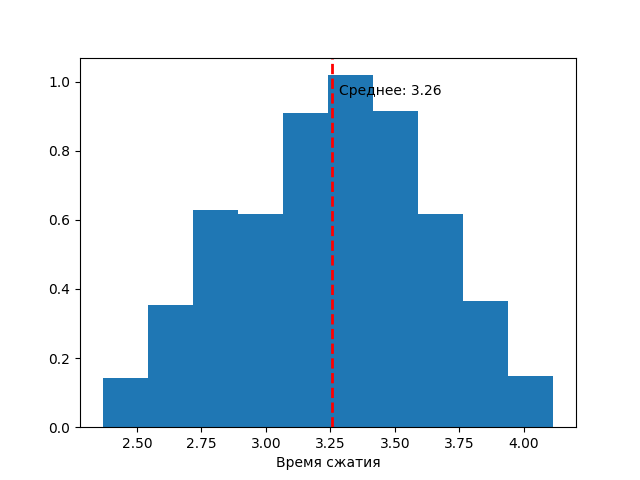
\includegraphics{images/hist-exec-py-dev.png}
    \end{adjustbox}
    \caption{Время сжатия Python-устройством через подпроцесс.}\label{fig:hist-exec-py-dev}
\end{figure}



\chapter{Программный код}\label{app:B}

Proof Of Concept реализация {\mylanguage}, \cref{lst:core.template.c,lst:main.py,lst:schema_parser.py}.

\begin{lstlisting}[language={C},basicstyle=\tiny,stepnumber=1,caption={Шаблон устройства},label={lst:core.template.c}]
#include "qemu/osdep.h"
#include "qapi/error.h"
#include "qom/object.h"
/*[[[cog
    import json as j
    import main as m

    with open(m.DEV_SCHEMA_FILE, 'r') as sf:
        SCHEMA = j.load(sf)

    device_header = SCHEMA["parent"]["header"]
    cog.outl(f'#include "{device_header}"')
   ]]]*/
/*[[[end]]]*/
#include "exec/address-spaces.h"
#include "hw/qdev-properties-system.h"

#include <Python.h>

#define IF_NULL_GOTO_ERR(VAR, BODY) \
    BODY; \
    if (!VAR){ \
        goto err; \
    }

#define PY_COMPILE_AND_GET_FUNC(FUNC_NAME, PY_CODE, PY_COMPILED, PY_MODULE, PY_FUNC) \
    if (!PY_COMPILED){ \
        IF_NULL_GOTO_ERR(PY_COMPILED, \
                         PY_COMPILED = Py_CompileString(PY_CODE, FUNC_NAME ".py", Py_single_input)) \
    } \
    IF_NULL_GOTO_ERR(PY_MODULE, \
                     PY_MODULE = PyImport_ExecCodeModule(FUNC_NAME "module", PY_COMPILED)) \
    IF_NULL_GOTO_ERR(PY_FUNC, \
                     PY_FUNC = PyObject_GetAttrString(PY_MODULE, FUNC_NAME))


typedef struct {
    char *name;
    size_t size;
} DeviceFieldMetaInfo;


/*[[[cog
    #
    # generating device class
    #

    import json as j
    import main as m
    from textwrap import indent, dedent
    INDENT = lambda s: indent(s, ' '*4)

    with open(m.DEV_SCHEMA_FILE, 'r') as sf:
        SCHEMA = j.load(sf)


    device_class    = m.get_device_class_name(SCHEMA, full = True)
    device_instance = m.get_device_class_name(SCHEMA)
    device_parent   = SCHEMA["parent"]["name"]


    cog.outl("typedef struct {")
    cog.outl(INDENT(f"{device_parent}Device parent_obj;"))
    cog.outl(f"}} {device_class};")
    cog.outl()
    cog.outl(f"typedef struct __attribute__((packed)) {{")
    for fname, ftype in m.get_nested_schema(SCHEMA, "device").items():
        cog.outl(INDENT(f"{ftype} {fname};"))
    cog.outl(f"}} {device_instance};")

    cog.outl()
    cog.outl()
    cog.outl(f"DeviceFieldMetaInfo device_fields[] = {{")
    for fname, ftype in m.get_nested_schema(SCHEMA, "device").items():
        cog.outl(INDENT(f'{{ "{fname}", sizeof({ftype}) }},'))
    cog.outl(INDENT('};'))
  ]]]*/
/*[[[end]]]*/

#define DEVICE_FIELDS_COUNT sizeof(device_fields)/sizeof(device_fields[0])

static PyObject* create_dict_for_class_fields(){
    PyObject* p_field_dicts[DEVICE_FIELDS_COUNT];
    PyObject *p_meta_info_aggregation = PyDict_New();
    for(int i = 0; i < DEVICE_FIELDS_COUNT; i++){
        int err = PyDict_Merge(p_meta_info_aggregation,
                               Py_BuildValue("{s:i}",
                                             device_fields[i].name,
                                             device_fields[i].size),
                               1);
        if(err){
            PyErr_Print();
            abort();
        }
    }
    return p_meta_info_aggregation;
}

PyObject *DictWithClassFields;

/*[[[cog
    #
    # generating device type
    #

    import json as j
    import main as m

    with open(m.DEV_SCHEMA_FILE, 'r') as sf:
        SCHEMA = j.load(sf)

    device_instance    = m.get_device_class_name(SCHEMA)
    device_name        = SCHEMA["name"]
    device_parent_type = SCHEMA["parent"]["type"]
    device_interface   = SCHEMA["parent"]["interface"]
    device_qtype       = SCHEMA["name"].upper()

    cog.outl(f'#define TYPE_{device_qtype} "{device_name}"')
    cog.outl(f"""OBJECT_DEFINE_TYPE_WITH_INTERFACES({device_instance},
                                       {device_name},
                                       {device_qtype},
                                       {device_parent_type}_DEVICE,
                                       {{ INTERFACE_{device_interface} }},
                                       {{ NULL }})""")
  ]]]*/
/*[[[end]]]*/

/*[[[cog
    #
    # generating function prototypes
    #

    import json as j
    import main as m
    from textwrap import indent, dedent
    INDENT = lambda s: indent(s, ' '*4)

    with open(m.DEV_SCHEMA_FILE, 'r') as sf:
        SCHEMA = j.load(sf)

    class_methods = SCHEMA["class"]["schema"]["methods"]
    class_init = m.create_device_method_proto(SCHEMA, "void", "class_init", "ObjectClass *oc, void *data")
    cog.outl(f"{class_init};")

    for method in class_methods:
        cog.outl(f'{m.create_device_method_proto(SCHEMA, method["c_ret"], method["c_name"], method["c_args"])};')
  ]]]*/
/*[[[end]]]*/

/*[[[cog
    #
    # generating device properties
    #

    import json as j
    import main as m
    from textwrap import indent, dedent
    INDENT = lambda s: indent(s, ' '*4)

    with open(m.DEV_SCHEMA_FILE, 'r') as sf:
        SCHEMA = j.load(sf)

    device_name = SCHEMA['name']

    cog.outl(f"static Property {device_name}_properties[] = {{")
    for p in m.get_nested_schema(SCHEMA, 'properties'):
        ptype         = p["type"].upper()
        pname         = f"\"{p['name']}\""
        pfield        = p["field"]
        dev_name      = m.get_device_class_name(SCHEMA)
        default_value = ''

        if "default_value" in p:
            default_value = ', ' + str(p["default_value"])

        cog.outl(INDENT(f"DEFINE_PROP_{ptype}({pname}, {dev_name}, {pfield}{default_value}),"))
    cog.outl(INDENT("DEFINE_PROP_END_OF_LIST()"))
    cog.outl("};")
  ]]]*/
/*[[[end]]]*/

/*[[[cog
    #
    # generating device MemoryRegionOps
    #

    import json as j
    import main as m
    from textwrap import indent, dedent
    INDENT = lambda s: indent(s, ' '*4)

    with open(m.DEV_SCHEMA_FILE, 'r') as sf:
        SCHEMA = j.load(sf)

    device_name = SCHEMA['name']

    for k,v in m.get_nested_schema(SCHEMA, "device").items():
        if v == "MemoryRegionOps":
            cog.outl(f"static const MemoryRegionOps {device_name}_mem_ops = {{")
            for mem_k, mem_v in SCHEMA["device"]["schema"][k].items():
                cog.outl(INDENT(f".{mem_k} = {mem_v},"))

            cog.outl(INDENT(f".read = {m.get_method_name(SCHEMA, 'read')},"))
            cog.outl(INDENT(f".write = {m.get_method_name(SCHEMA, 'write')},"))

            cog.outl("};")
  ]]]*/
/*[[[end]]]*/

/*[[[cog
    #
    # generating device and instance methods
    #

    import re
    import json as j
    import main as m

    from textwrap import indent, dedent
    INDENT = lambda s: indent(s, ' '*4)
    ALIGN_INDENT_BY = lambda s: ' ' * len(s)

    with open(m.DEV_SCHEMA_FILE, 'r') as sf:
        SCHEMA = j.load(sf)


    device_name      = SCHEMA["name"]
    class_init_proto = m.create_device_method_proto(SCHEMA, "void", "class_init", "ObjectClass *oc, void *data")

    cog.outl(f"{class_init_proto}{{")

    class_field_init = SCHEMA["class"]["schema"]["init"]["class_field_init"]

    if not any(filter(lambda cast: cast["dev_cast"]["type"] == "DeviceClass",
                      class_field_init)):
        default_dev_cast = {"dev_cast": {"type" : "DeviceClass", "cast": "DEVICE_CLASS"}}
        class_field_init = [default_dev_cast] + class_field_init

    for entry in class_field_init:
        cog.outl()
        dev_cast   = entry["dev_cast"]
        cast_type  = dev_cast['type']
        cast_macro = dev_cast['cast']

        cog.outl(INDENT(f"{cast_type} *{cast_type}_ptr = {cast_macro}(oc);"))

        for k,v in entry.items():
            if k == "dev_cast":
                continue
            cog.outl(INDENT(f"{cast_type}_ptr->{k} = {v};"))


    cog.outl(INDENT(f"device_class_set_props(DeviceClass_ptr, {device_name}_properties);"))

    cog.outl()
    cog.outl(INDENT(f'Py_SetProgramName("{device_name}");'))
    cog.outl(INDENT(f'Py_Initialize();'))
    cog.outl(INDENT(f'DictWithClassFields = create_dict_for_class_fields();'))
    cog.outl("}")
    cog.outl()
    cog.outl()

    for method in class_methods:
        method_proto = m.create_device_method_proto(SCHEMA, method["c_ret"], method["c_name"], method["c_args"])
        argc = method["c_args"].count(',') + 1
        arguments = [s.strip() for s in method["c_args"].split(',')]
        casts = [s.strip() for s in method["c_to_py_cast"].split(',')]

        argument_type_val = [arg.split() for arg in arguments]
        arguments_and_cast = list(zip(argument_type_val, casts))

        if len(argument_type_val) != len(arguments_and_cast):
            cog.error(f"{argument_type_val} and {casts} length mismatch!")

        cog.outl(f"{method_proto}{{")

        pass_args_to_python = ''
        memoryview_vars = []
        for i, (arg, cast) in enumerate(arguments_and_cast):
            is_pointer = '*' in arg[0] + arg[1]
            arg_val = arg[1].replace('*', '')
            if is_pointer:
                arg_val_as_buf = arg_val
            else:
                arg_val_as_buf= '&' + arg_val

            if method["c_name"] == "realize" and \
               "MemoryRegionOps" in m.get_nested_schema(SCHEMA, "device").values():
                device_fields = m.get_nested_schema(SCHEMA, "device")
                reverse_device_fields = dict(zip(device_fields.values(), device_fields.keys()))
                mem_io_field = reverse_device_fields["MemoryRegionOps"]
                cog.outl(INDENT(f"memory_region_init_io(&(({cast}*){arg_val_as_buf})->{mem_io_field},"))
                cog.outl(INDENT(f"                      OBJECT({arg_val_as_buf}),"))
                cog.outl(INDENT(f"                      &{device_name}_mem_ops,"))
                cog.outl(INDENT(f"                      {arg_val_as_buf},"))
                cog.outl(INDENT(f'                      "{device_name}-mmio",'))
                cog.outl(INDENT(f"                      1);"))

            memoryview_vars.append(f"p_mem_view_{arg_val}")
            pass_args_to_python += INDENT(INDENT(dedent(f"""
                                                 PyObject *p_mem_view_{arg_val} = PyMemoryView_FromMemory((char*){arg_val_as_buf},
                                                                                                 {ALIGN_INDENT_BY(arg_val)}sizeof({cast}),
                                                                                                 {ALIGN_INDENT_BY(arg_val)}PyBUF_WRITE);
                                                 if (!p_mem_view_{arg_val}){{
                                                     goto err;
                                                 }}
                                                 PyTuple_SetItem(p_func_args, {i}, p_mem_view_{arg_val});
                                                 """)))

            memoryview_vars_free = INDENT('\n'.join([f'Py_XDECREF({mv});' for mv in memoryview_vars]))
            py_return_code = ''
            py_return_val_name = ''
            if method["c_ret"] != "void":
                py_return_val_name = 'py_out'
                py_return_code = INDENT(dedent(f"""
                                        char *py_out_buf;
                                        {method["c_ret"]} {py_return_val_name};
                                        int ok = PyArg_ParseTuple(p_ret, "S", &py_out_buf);
                                        {py_return_val_name} = *({method["c_ret"]}*)py_out_buf;
                                        """))

        pass_args_to_python += INDENT(INDENT(f"PyTuple_SetItem(p_func_args, {argc}, DictWithClassFields);\n"))
        c_function_body = m.get_python_c_api_wrap(SCHEMA,
                                                  'class',
                                                  method["py_name"],
                                                  argc + 1,
                                                  pass_args_to_python,
                                                  return_val=py_return_val_name)
        if method["c_name"] == "finalize":
            err_handling_code = "if(Py_FinalizeEx()){\n" \
                                + INDENT(INDENT("PyErr_Print();\n")) \
                                + INDENT(INDENT("abort();\n")) \
                                + INDENT("}\n")
            c_function_body = re.sub("//.*?\n",
                                     err_handling_code + memoryview_vars_free + '\n',
                                     c_function_body)
        else:
            c_function_body = re.sub("\s+//.*?\n", f"\n{py_return_code}\n{memoryview_vars_free}\n", c_function_body, count=1)
            c_function_body = re.sub("\s+//.*?\n", f"\n{memoryview_vars_free}\n", c_function_body, count=1)
        c_function_body = '\n'.join(filter(lambda l: not re.match("\s+$", l), c_function_body.splitlines()))
        cog.outl(c_function_body)

        cog.outl("}")
        cog.outl()
        cog.outl()
  ]]]*/
/*[[[end]]]*/
\end{lstlisting}


\begin{lstlisting}[language={Python},basicstyle=\tiny,stepnumber=1,caption={Вспомогательные методы кодогенерации},label={lst:main.py}]
import os
import sys
import json
import inspect
import importlib.util
import subprocess as subp

from pathlib import Path
from textwrap import dedent

import schema_parser as sp


def get_nested_schema(schema: dict, key: str):
    return schema[key]['schema'][key]


def get_device_class_name(schema: dict, full=False):
    base_class_name = schema["name"].replace('_', ' ').title().replace(' ', '')
    if full:
        return base_class_name + "Class"
    return base_class_name


def get_function_text_from(sub_schema: dict, method_name: str):
    spec = importlib.util.spec_from_file_location("py_code", sub_schema["code"])
    py_code = importlib.util.module_from_spec(spec)
    spec.loader.exec_module(py_code)
    return inspect.getsource(getattr(py_code, method_name)).split('\n')


def get_python_c_api_wrap(schema: dict,
                          _from: str,
                          func_name: str,
                          tuple_size: int,
                          code_for_insert: str,
                          return_val: str = ''):
    c_char_source = [l + '\\n' for l in get_function_text_from(schema[_from], func_name)]

    py_code = f"static char *py_code = "
    py_code_start = len(py_code) + 8

    py_code += f'"{c_char_source[0]}"\n'
    for line in c_char_source[1:-1]:
        py_code += py_code_start*' ' + f'"{line}"\n'
    py_code += py_code_start*' ' + f'"{c_char_source[-1]}";'

    check_code = """if (!{what}){{
            goto err;
        }}"""

    return dedent(f"""
        {py_code}
        static PyObject *p_compiled_code = NULL;
        PyObject *p_module = NULL,
                 *p_func = NULL,
                 *p_func_args = NULL,
                 *p_ret = NULL;

        PY_COMPILE_AND_GET_FUNC("{func_name}",
                                py_code,
                                p_compiled_code,
                                p_module,
                                p_func);

        p_func_args = PyTuple_New({tuple_size});
        {check_code.format(what='p_func_args')}
        {code_for_insert}
        p_ret = PyObject_CallObject(p_func, p_func_args);
        {check_code.format(what='p_ret')}

        // for post creation code insert
        Py_XDECREF(p_module);
        Py_XDECREF(p_func);
        Py_XDECREF(p_func_args);
        Py_XDECREF(p_ret);
        return {return_val};

    err:
        PyErr_Print();
        // for post creation code insert
        Py_XDECREF(p_module);
        Py_XDECREF(p_func);
        Py_XDECREF(p_func_args);
        Py_XDECREF(p_ret);
        abort();
        """)


def get_method_name(schema: dict,
                    method_name: str):
    return f"{schema['name']}_{method_name}"


def create_device_method_proto(schema: dict,
                               ret_type: str,
                               method_name: str,
                               args: str,
                               static=True):
    method_proto = f"{ret_type} {get_method_name(schema, method_name)}({args})"
    if static:
        return f"static {method_proto}"
    return method_proto


DEV_SCHEMA_FILE = 'concrete_dev_schema.json'

if __name__ == '__main__':
    ENV = os.environ.copy()
    ENV["PYTHONPATH"] = Path('.').absolute()
    SCHEMA = sp.load_schema(sys.argv[1])

    with open(DEV_SCHEMA_FILE, 'w') as cds:
        json.dump(SCHEMA, cds, indent=2)


    subp.run(['cog', '-d', '-o', SCHEMA["name"] + '.c', sys.argv[2]],
             env=ENV)
\end{lstlisting}


\begin{lstlisting}[language={Python},basicstyle=\tiny,stepnumber=1,caption={Парсер схемы},label={lst:schema_parser.py}]
import json
import typing as t

from pathlib import Path


def load_schema(filename: str):
    schema_path = Path(filename)

    def get_load_path(path: Path):
        return path if path.is_absolute() else schema_path.parent / path

    def load_into_schema(schema_slice: dict,
                         key: str,
                         path: Path,
                         as_json=True):
        with open(path, 'r') as f:
            if as_json:
                schema_slice[key] = json.load(f)
            else:
                schema_slice[key] = f.read()


    with open(schema_path, 'r') as f:
        init_schema = json.load(f)
        for k in filter(lambda k: type(init_schema[k]) == dict and \
                                  'schema' in init_schema[k] and \
                                  'code' in init_schema[k], init_schema):
            subschema_path = get_load_path(Path(init_schema[k]['schema']))
            subschema_code = get_load_path(Path(init_schema[k]['code']))
            load_into_schema(init_schema[k], 'schema', subschema_path)
            init_schema[k]['code'] = str(subschema_code)

    return init_schema
\end{lstlisting}
